\documentclass[11pt,a4paper,french]{article}
\usepackage{babel}
\usepackage[T1]{fontenc}
\usepackage[utf8]{inputenc}
\usepackage{amssymb,amsmath,amscd,pdfsync}
\usepackage{stmaryrd}
\usepackage{enumerate}
\usepackage[a4paper,margin=15mm,includehead]{geometry}
\usepackage{tikz}
\usetikzlibrary{positioning}
\usepackage{fancyhdr}
\usepackage{paracol}
\usepackage{listings}

% symboles fr pour leq et geq
\newcommand{\Leq}{\leqslant}
\newcommand{\Geq}{\geqslant}

% Environnement question, similaire à celui su sujet d'origine.
\newcounter{numQ}
\newcommand{\debquestion}{\refstepcounter{numQ}
  \columnratio{0.07}
  \medskip
  \paracol{2}
  \textbf{Q\arabic{numQ}}
  \switchcolumn
  \noindent}
\newcommand{\finquestion}{\endparacol\medskip}
\newenvironment{question}{\debquestion}{\finquestion}

% pour les algorithmes en pseudo-code
\lstdefinelanguage{pseudoCode}{
  morekeywords={Entrees, Sorties, Algorithme, pour, finPour, faire, tantQue, finTantQue, si, alors, sinon, finSi, sortir, retourner},
  morecomment=[l]{//}
}  
\lstset{basicstyle=\ttfamily,
  language=pseudoCode,
  keywordstyle=\bfseries\color{black}\sffamily,
  % À DÉCOMMENTER SI VOUS VOULEZ INSÉRER DES NUMÉROS DE LIGNE
  %numbers=left, %numbers
  %numberstyle=\tiny, %numbers
  %stepnumber=2, %numbers
  %numbersep=5pt, %numbers
  mathescape,
  inputencoding=utf8,
  extendedchars=trueinputencoding=utf8,
  extendedchars=true,  
  literate=
  {é}{{\'{e}}}1
  {è}{{\`{e}}}1
  {à}{{\`{a} }}1
  {ç}{{\c{c}}}1
  {œ}{{\oe}}1
  {ù}{{\`{u}}}1
  {É}{{\'{E}}}1
  {È}{{\`{E}}}1
  {À}{{\`{A}}}1
  {Ç}{{\c{C}}}1
  {Œ}{{\OE}}1
  {Ê}{{\^{E}}}1
  {ê}{{\^{e}}}1
  {î}{{\^{i}}}1
  {ô}{{\^{o}}}1
  {û}{{\^{u}}}1
  {ë}{{\¨{e}}}1
  {û}{{\^{u}}}1
  {â}{{\^{a}}}1
  {Â}{{\^{A}}}1
  {Î}{{\^{I}}}1
}
\renewcommand{\lstlistingname}{Algorithme}

%quelques macros de maths
\newcommand{\R}{\mathbb{R}}
\newcommand{\N}{\mathbb{N}}
\newcommand{\eps}{\epsilon}
\newcommand{\e}{\mathrm{e}}
\renewcommand{\O}[1]{\mathcal{O}\left( #1 \right)}


%Titre
\pagestyle{fancy}
\lhead{Épreuve d'informatique}
\chead{CCINP}
\rhead{\thepage/9}
\lfoot{}
\rfoot{}
\cfoot{MPI 2023}

\begin{document}

\begin{center}
  {\large
    Épreuve mutualisée avec E3A - Polytech \linebreak
    Épreuve spécifique - Filière MPI \linebreak
    \hrule
    \vspace{0.5cm}
    \textbf{Informatique} \linebreak
    \textbf{Durée : 4h} \linebreak
    \hrule
  }
\end{center}
N.B. : le candidat attachera la plus grande importance à la clarté, à la précision et à la concision de la rédaction. Si un candidat est amené à reprérer ce qui peut lui sembler être une erreur d'énoncé, il le signalera sur sa copie et devra poursuivre sa composition en expliquant les raisons des initiatives qu'il a été amené à prendre.
\vspace{2cm}
\begin{center}
  RAPPEL DES CONSIGNES \linebreak
\end{center}
\begin{itemize}
\item Utiliser uniquement un stylo noir ou bleu foncé non effaçable pour la rédaction de votre composition ; d'autres couleurs, excepté le vert, peuvent être utilisées, mais uniquement pour les schémas et la mise en évidence des résultats.
\item Ne pas utiliser de correcteur.
\item Écrire le mot FIN à la fin de votre composition.
\end{itemize}
\begin{center}
  \vspace{1cm}
  Les calculatrices sont interdites. \linebreak
  \vspace{2cm}
  Le sujet est composé de trois parties, toutes indépendantes.
\end{center}

\newpage

\section{Palindromes}

En langue française, "ressasser" est le mot palindrome le plus long, tandis qu'il semble que "saippuakauppias" soit le plus long mot palinfrome au monde, désignant un marchand de savon en Finlande. L'objet de cette partie est de compter le nombre de palindromes présents dans un mot donné.

Soit $\Sigma$ un alphabet fini contenant au moins deux lettres. on note $u = u_0 \dots u_{n-1}$ un \emph{mot} sur $\Sigma$, composé de $n$ lettres $u_i \in \Sigma, i \in \llbracket 0; n - 1 \rrbracket$. La longueur de $u$ est notée $|u|$. Pour $0 \Leq i < j \Leq n$, on note $u[i,j]$ le mot $u_i \dots u_{j-1}$. L'ensemble des mots construit sur $\Sigma$ et contenant le mot vide $\eps$ est noté $\Sigma^*$.

\medskip

\textbf{Définition 1} (Miroir)

Soit $u \in \Sigma^*$. Le \emph{miroir} de $u = u_0 \dots u_{n-1}$, noté $\overline{u}$, est le mot $\overline{u} = u_{n-1} \dots u_0$. Par convention $\overline{\eps} = \eps$.

\medskip

\textbf{Définition 2} (Palindrome)

$u \in \Sigma^*$ est un \emph{palindrome} si et seulement si $u = \overline{u}$.

\medskip

Par convention, le mot vide $\eps$ n'est pas considéré comme un palindrome.

On dira qu'un palindrome $u$ est \emph{pair} (respectivement \emph{impair}) lorsque sa longueur $|u|$ est paire (resp. impaire).

On recherche donc dans cette partie le nombre de palindromes facteurs d'un mot $u \in \Sigma^*$ (comptés avec les mulitplicités éventuelles), soit le cardinal de l'ensemble $\left\{ (i,j), 0 \Leq i < j \Leq |u|, u[i,j] = \overline{u[i,j]} \right\}$. Dit autrement, on recherche le nombre de palindromes contenus dans $u$.

\begin{question}
  Si $\Sigma = \{a,b\}$, donner le nombre de palindromes contenus dans le mot $u = babb$.
\end{question}

En parcourant naïvement les lettres d'un mot $u$ donné, on peut proposer un algorithme en pseudo-code permettant de compter naïvement les palindromes de $u$ (\textbf{algorithme~\ref{algo_naif}}).

\begin{lstlisting}[caption={Décompte naïf du nombre de palindromes contenu dans un mot donné},
    label=algo_naif]
 Entrees : Un mot $u$.
 Sorties : Le nombre de palindromes contenus dans $u$.
 Algorithme :
  nb = 0
  pour $i$ = 0 à $|u| - 1$ faire
    pour $j$ = 0 à $|u| - 1$ faire
      estPalindrome = True
      pour $k$ = $i$ à $j - 1$ faire
        si $u[i] \not = u[j - k - 1]$ alors 
          estPalindrome = False
          sortir du pour $k$
        finSi
      finPour    
      si estPalindrome alors
        nb = nb + 1    
      finSi
    finPour
  finPour
  retourner nb
\end{lstlisting}
% note : je me suis permis d'adapter un peu la présentation de l'énoncé (avec des finSi et finPour) étant donné que je ne sais pas faire des lignes d'indentation avec listings.

\begin{question}
  Évaluer la complexité au pire des cas de l'\textbf{algorithme~\ref{algo_naif}} en fonction de $|u|$.
\end{question}

\newpage

On souhaite bien sûr améliorer cette première idée. Pour ce faire, on utilise tout d'abord le paradigme de la programmation dynamique.

Pour $u \in \Sigma^*$, on définit un tableau de booléens $P$ de taille $(|u| + 1) \times (|u| + 1)$, $P[i][j]$ étant vrai si $u[i,j]$ est un palindrome. on a donc pour tout $i \in \llbracket 0, |u| - 1 \rrbracket$, $P[i][i+1] = \text{True}$.

\begin{question}
  Soit $u[i,j]$ un mot. À quelles conditions sur $u_i$, $u_{j-1}$ et $u[i+1,j-1]$ le mot $u[i,j]$ est-il un palindrome ?
\end{question}

\begin{question}
  En déduire une relation de récurrence vérifiée par les coefficients de $P$.
\end{question}

\begin{question}
  Écrire un algorithme de programmation dynamique en pseudo-code résolvant le problème. Évaluer sa complexité.
\end{question}

On insère maintenant entre chaque paire de lettres de $u$, ainsi qu'au début et à la fin du mot, un symbole spécial noté $\#$. On appelle ce nouveau mot $u^{\#}$. Ainsi, le mot $u = abba$ se transforme en $u^{\#} = \#a\#b\#b\#a\#$.

\begin{question}
  Montrer que les palindromes de $u^{\#}$, s'ils existent, sont tous impairs.
\end{question}

\begin{question}
  Soit $v$ un palindrome de longueur $2k + 1$ de $u$, $k \in \N$ On construit le mot $u^{\#}$. Donner les deux palindromes correspondant à $v$ dans $u^{\#}$.
\end{question}

\begin{question}
  Même question si $v$ est un palindrome de longueur $2k$ de $u$.
\end{question}


\begin{question}
  En déduire une stratégie de recherche de tous les palindromes de $u$.
\end{question}

On voit que les palindromes impairs sont importants. On va donc construire un algorithme de recherche de ce type de palindrome.

\medskip

\textbf{Définition 3} (Rayon d'un palindrome)

Soient $u \in \Sigma^*$ et $i \in \llbracket 0, |u| - 1 \rrbracket$. On dit qu'il existe un \emph{palindrome centré en $i$ de rayon $\rho > 0$} si :
\begin{enumerate}[(i)]
\item $i - \rho \Geq 0$,
\item $i + \rho + 1 \Leq |u|$,
\item $u[i - \rho, i + \rho + 1]$ est un palindrome.
\end{enumerate}

Le \emph{rayon maximal} $\hat{\rho}_i$ d'un palindrome centré en $i$ est le plus grand rayon d'un palindrome centré en $i$.

\medskip

Par exemple, si $u = abbababab$ et $i = 4$, alors $b$ est un palindrome centré en $4$ de rayon $0$, $aba$ est un palindrome centré en $4$ de rayon $1$, $babab$ est un palindrome centré en $4$ de rayon $2$ et c'est le lus grand, donc $\hat{\rho}_4 = 2$.

\begin{question}
  En remarquant qu'un palindrome impair est centré sur une lettre (ou un symbole spécial dans le cas de $u^{\#}$), proposer un algorithme en pseudo-code permettant de compter le nombre de palindromes impairs d'un mot $u$. Évaluer sa complexité.
\end{question}

\begin{question}
  Soient $u \in \Sigma^*, i \in \llbracket 0, |u|-1 \rrbracket$ et $j \in \llbracket 1,\hat{\rho}_i \rrbracket$. En exploitant les différentes symétries, montrer qu'il existe un palindrome centré en $i + j$ de rayon $\min(\hat{\rho}_i-j,\hat{\rho}_{i-j})$. En déduire  \newline $\hat{\rho}_{i+j} \Geq \min(\hat{\rho}_i-j,\hat{\rho}_{i-j})$. Préciser à quelle condition il y a égalité.
  % ERREUR SUJET :
  % Un 0 < en trop à la première ligne
\end{question}
    
En utilisant cette remarque, on développe un algorithme, dit de Manacher, qui construit un tableau d'entiers $T$ permettant de compter le nombre de palindromes d'un mot $u$. Plus précisément, pour chaque position $i \in \llbracket 1, |u| - 1 \rrbracket$, $T[i]$ indique le rayon maximal $\hat{\rho}_i$, donc tel que la sous-chaîne de $i-\hat{\rho}_i$ à $i + \hat{\rho}_i + 1$ est un palindrome. L'\textbf{algorithme~\ref{algo_manacher}} consiste à incrémenter $T[i]$ jusqu'à trouver le plus grand palindrome $u[i - T[i], i + T[i] + 1]$ centré en $i$.
% ERREUR SUJET :
% une erreur de signe ($i - ρ_i + 1$ au lieu de $i + ρ_i + 1$)
% un + en trop à la dernière ligne

\newpage

\begin{lstlisting}[caption={Algorithme de Manacher},
    label=algo_manacher]
 Entrees : Un mot $u$.
 Sorties : Un tableau $T$.
 Algorithme :
  Initialiser un tableau $T$ de $|u|$ cases, initialisées à 0
  $k$ = 0
  pour $i$ = 1 à $|u| - 1$ faire
    $j$ = $i - k$
    si $T[k] \Geq j$ alors
      $T[i]$ = $\min(T[k-j],T[k] - j)$
    finSi
    tantQue $(i - (T[i] + 1)) \Geq 0$ ET $(i - (T[i] + 1)) < |u|$ ET $u[i - (T[i] + 1)] = u[i + T[i] + 1]$ faire
      $T[i]$ = $T[i]+1$
      $k = i$
    finTantQue
  finPour
  retourner $T$
\end{lstlisting}

\begin{question}
  Comment trouver à partir de cet algorithme le nombre de palindromes de $u$ ?
\end{question}

\begin{question}
  Quelle est la complexité de cet algorithme ? Justifier.
\end{question}

\section{Traversée de rivière}

Cette partie comporte des questions nécessitant un \textbf{code Ocaml}.

Dans une vallée des Alpes, un passage à gué fait de cailloux permet de traverser la rivière. Deux groupes de randonneurs arrivent simultanément sur les berges gauche et droite de cette rivière et veulent la traverser. Le chemin étant très étroit, une seule personne peut se trouver sur chaque caillou de ce chemin (\textbf{figure~\ref{randonneurs}}). Un randonneur sur la berge de gauche peut avancer d’un caillou (vers la droite sur la \textbf{figure~\ref{randonneurs}}) et sauter par dessus le randonneur devant lui (un caillou à droite) si le caillou où il atterit
est libre. De même, chaque randonneur de la berge de droite peut avancer d’un caillou (vers la gauche sur la \textbf{figure~\ref{randonneurs}}) et sauter par dessus le randonneur devant lui, dans la mesure où le caillou sur lequel il atterit est libre. Une fois engagés, les randonneurs ne peuvent pas faire marche arrière. De plus, pour simplifier, on suppose qu’une fois tous les randonneurs sur le chemin, il ne reste qu’un caillou de libre.

\begin{figure}[h]
  \begin{center}
    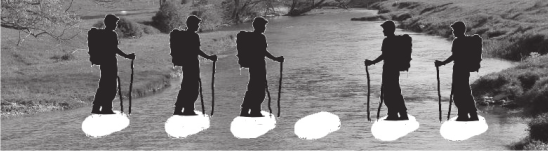
\includegraphics{randonneurs.png}
    \caption{Les randonneurs et le chemin de cailloux.\label{randonneurs}}
  \end{center}
\end{figure}

Le chemin de cailloux est défini par un tableau d'entiers :

\begin{center}
  \verb|type chemin_caillou = int array|
\end{center}

Dans ce tableau, un randonneur venant de la berge de gauche est représenté par un $1$, un randonneur issu de la berge de droite par un $2$, et un caillou libre par un $0$.

\quad

\begin{question}
  Écrire une fonction de signature \verb|caillou_vide : chemin_caillou -> int| qui détermine la position du caillou inoccupé.
  
\end{question}

\begin{question}
  Écrire une fonction de signature \verb|echange : chemin_caillou -> int -> int -> chemin_caillou| qui permute les valeurs codées sur deux cailloux. Le tableau d'entiers initial représentant le chemin n'est pas modifié. On pourra utiliser ici la fonction \verb|copy| du module \verb|Array|.
\end{question}

\begin{question}
  Écrire une fonction de signature \verb|randonneurG_avance : chemin_caillou -> bool| qui teste si, parmi les randonneurs venant de la berge de gauche, il en existe un qui puisse avancer (vers la droite).
\end{question}

\begin{question}
  Écrire une fonction de signature \verb|randonneurG_saute : chemin_caillou -> bool| qui teste si, parmi les randonneurs venant de la berge de gauche, il en existe un qui puisse sauter (vers la droite) au-dessus d'un randonneur.
\end{question}

  On supposera dans la suite les fonctions de signature \verb|randonneurD_avance : chemin_caillou -> bool| et \verb|randonneurD_saute : chemin_caillou -> bool| écrites de manière similaire pour les randonneurs venant de la berge de droite.

\begin{question}
  Écrire une fonction de signature \verb|mouvement_chemin : chemin_caillou -> chemin_caillou list| qui, en fonction de létat du chemin, calcule l'état suivant après les opérations suivantes (si elles sont permises) :
  \begin{enumerate}[(i)]
  \item déplacement d'un randonneur venant de la berge de gauche,
  \item déplacement d'un randonneur venant de la berge de droite,
  \item saut d'un randonneur venant de la berge de gauche,
  \item saut d'un randonneur venant de la berge de droite.
  \end{enumerate}

  On donne la syntaxe OCaml pour crréer une liste de $N$ entiers $i$ : \verb|List.init N (fun x -> i)|.

  Par exemple, \verb|List.init 5 (fun x -> 2);;| renvoie \verb|[2;2;2;2;2]|.
\end{question}

\begin{question}
  Écrire une fonction de signature \verb|passage : int -> int -> chemin_caillou list|, utilisant la question précédente, telle que l'appel \verb|passage nG nD| résout le problème du passage de \verb|nG| randonneurs venant de la berge de gauche et \verb|nD| randonneurs venant de la berge de droite. Par exemple, \verb|passage 3 2| permet de passer de \verb|[1;1;1;0;2;2]| à \verb|[2;2;0;1;1;1]|.
  % ERREUR SUJET :
  % j'ai fait une supposition sur le type attendu de la fonction qui ne pouvait pas être int -> int
\end{question}

\section{Calcul d'une coupe minimu d'un graphe}

Un agent secret a pour mission de perturber le réseau de communications ennemi en coupant certains fils dans le réseau. Ayant peu de moyens, l’agent a pour consigne de couper le moins de fils possibles pour accomplir cette tâche. Le réseau de communications est modélisé à l’aide d’un \emph{multigraphe} non orienté $G = (S , A)$, où $S$ est l’ensemble des sommets du graphe et $A$ l’ensemble de ses arêtes. Résoudre le problème de l’agent secret, c’est rechercher une \emph{coupe minimum} dans $G$.

\medskip

\textbf{Définition 4} (Multigraphe)

Un multigraphe est un graphe dans lequel des couples de mêmes sommets peuvent être reliés par plus d’une arête.

\medskip

Dans toute la suite, on considérera les multigraphes sans arêtes du type $(s, s)$ (boucles).

\medskip

\textbf{Définition 5} (Coupe)

Une coupe d’un multigraphe non orienté $G = (S , A)$ est une partition non triviale $(S_1 , S_2)$ de $S$, c’est-à-dire telle que $S_1 \cup S_2 = S$ , $S_1 \cap S_2 = \emptyset$ et $S_1 , S_2 \not = \emptyset$. On dira que les arêtes reliant $S_1$ à $S_2$ sont les arêtes de la coupe.


La \emph{taille} d'une coupe $(S_1, S_2)$ est définie par $|(S_1,S_2)| = \left| \left\{ (s,t) \in A, s \in S_1, t in S_2 \right\} \right|$. Autrement dit, c'est le nombre d'arêtes de $G$ qui relient $S_1$ et $S_2$.

\medskip

\textbf{Définition 6} (Coupe minimum)

Une coupe minimum est une coupe de taille minimale.

\medskip

Pour trouver une coupe minimum d’un multigraphe $G = (S , A)$, on pourrait énumérer l’ensemble des coupes possibles (il y en a $2^{|S|}$...), ou encore utiliser un algorithme de flot (le plus efficace étant en $\O{|S|^3}$). Nous proposons dans la suite un algorithme probabiliste, l’algorithme de Karger, basé sur la notion de contraction d’arête.

\subsection{Contraction d'arête}

Soient $G = (S , A)$ un multigraphe et $a = (s, t) \in A$ une arête de $G$ de sommets $s$ et $t$. \emph{Contracter} l’arête $a$ consiste à :
\begin{enumerate}[i]
\item Créer un nouveau sommet $u = (st)$ dans $S$. $u$ est un \emph{supersommet} du nouveau graphe.
\item Pour toute arête $(r, s)$ ou $(r, t)$, $r \in S$ , ajouter une arête $(r, u)$ à $A$. Dans le cas où $(r, s)$ et $(r, t)$ existent, deux arêtes reliant $r$ à $u$ sont créées.
\item Supprimer de $A$ toutes les arêtes ayant $s$ ou $t$ comme extrémité.
\item Supprimer $s$ et $t$ de $S$.
\end{enumerate}

Un supersommet peut donc être vu comme un ensemble de deux sommets du graphe initial, obtenu après une contraction d’arête.

Le multigraphe obtenu est appelé \emph{graphe contracté} et est noté $G/st$. Si plusieurs arêtes relient $s$ à $t$ dans $G$, contracter l’une d’entre elles supprime toutes les autres du graphe $G/st$. Dans toute la suite, on notera $G_0$ le graphe initial, avant transformations par contractions.

On considère le graphe $G_0$ de la \textbf{figure~\ref{graphe_G0}}.

\begin{figure}[h]
  \begin{center}
    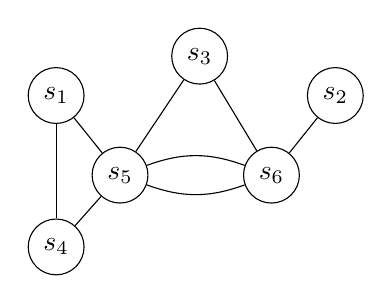
\begin{tikzpicture}[node distance = 1.2cm, every node/.style = {draw,circle}]
      \node (s1) {$s_1$};
      \node (s4) [below = of s1] {$s_4$}
      edge (s1);
      \node (s5) [below right = 0.5cm and 0.3cm of s1] {$s_5$}
      edge (s1)
      edge (s4);
      \node (s6) [right = of s5] {$s_6$}
      edge [out = 160, in = 20] (s5)
      edge [out = -160, in = -20] (s5);
      \node (s3) [above right = 1cm and 0.5cm of s5] {$s_3$}
      edge (s5)
      edge (s6);
      \node (s2) [above right = 0.5cm and 0.3cm of s6] {$s_2$}
      edge (s6);
      
    \end{tikzpicture}
  \end{center}
  \caption{Graphe $G_0$ exemple\label{graphe_G0}}
\end{figure}

\begin{question}
  Donner le graphe obtenu par contraction d’une arête $(s_5, s_6)$.
\end{question}

Après plusieurs contractions, un supersommet $u$ du graphe résultant contient un sous-ensemble $S_u \subseteq S$ de sommets de $G_0$.
% ERREUR SUJET
% G au lieu de  G_0.

\begin{question}
  Soit $u$ un supersommet et $s, t \in S_u$. Montrer qu’il existe un chemin $\Gamma$ entre $s$ et $t$ dans $G_0$ tel que chaque arête de $\Gamma$ a été contractée.
\end{question}

\begin{question}
  Montrer qu’en contractant une arête $s, t$ dans un multigraphe $G$, la taille d’une coupe minimum du graphe contracté $G/st$ est au moins égale à la taille d’une coupe minimum de $G$.
\end{question}

\begin{question}
  Montrer que la taille d’une coupe minimum de $G/st$ est strictement plus grande que celle d’une coupe minimum de $G$ si et seulement si l’arête $(s, t)$ est une arête de toutes les coupes minimum de $G$.
  \label{23}
\end{question}

\newpage

\subsection{Premier algorithme}

On construit un premier algorithme qui essaye de trouver une coupe minimum en contractant aléatoirement une arête de $G$, jusqu'à ce qu'il ne reste que deux sommets (\textbf{algorithme~\ref{algo_karger}}).

\begin{lstlisting}[caption={Algorithme de Karger},
    label=algo_karger]
Karger($G$, $n$)
Entrees : $G = (S , A)$ multigraphe non orienté, $n \in \N$
Sorties : Une coupe minimum de $G$.
Algorithme :
 pour $i$ = $|S|$ à $n$ en décrémentant de 1 faire
   Tirer aléatoirement (loi uniforme) une arête $a = (s, t) \in A$
   $G$ = $G/st$
 finPour
 retourner $G$

// Appel
Karger($G$, 2)
\end{lstlisting}
% ERREUR SUJET :
% J'ai ajouté un retour à cette fonction car sinon il manque clairement quelque chose...


\begin{question}
  Appliquer l’\textbf{algorithme~\ref{algo_karger}} au graphe de la \textbf {figure~\ref{graphe_G0}}, en contractant successivement $(s_5, s_6)$, $((s_5s_6), s_2)$, $(s_1, s_4)$ et $((s_5 s_6 s_2), s_3)$. Chaque graphe contracté sera représenté. La coupe calculée est-elle une coupe minimum ?
\end{question}

D’après la \textbf{Q\ref{23}}, tant que l’on ne contracte pas une arête faisant partie de toutes les coupes minimum de $G$, alors l’\textbf{algorithme~\ref{algo_karger}} trouvera une coupe minimum. On cherche alors la probabilité de ne  jamais contracter une telle arête.

\begin{question}
  Soit $d(s)$ le degré d’un sommet $s \in S$. Montrer que $\displaystyle \sum d(s) = 2|A|$ (lemme des poignées de main).
\end{question}

\begin{question}
  En déduire qu'une coupe minimum a une taille d'au plus $\dfrac{2|A|}{|S|}$.
\end{question}

Soit $C = (S_1,S_2)$ une coupe minimum de $G$. L’objet des questions \textbf{Q\ref{27}} et \textbf{Q\ref{28}} est de minorer la probabilité que l’\textbf{algorithme~\ref{algo_karger}} renvoie $C$. Pour cela, on remarque que cet algorithme ne renvoie pas $C$ si et seulement si lors d’une itération on choisit une arête qui traverse $C$, c’est-à-dire telle qu’un sommet est dans $S_1$ et l’autre dans $S_2$.

\begin{question}
  Quelle est la probabilité maximum de choisir une arête qui traverse $C$ ?
  \label{27}
\end{question}

\begin{question}
  En déduire que la probabilité $P_{|S|}$ que l’\textbf{algorithme~\ref{algo_karger}} renvoie $C$ est supérieure ou égale à $\dfrac{2}{|S|(|S| - 1)}$.
  \label{28}
\end{question}

\begin{question}
  Déduire de la question précédente qu’un multigraphe non orienté $G = (S , A)$ possède au plus $\dfrac{|S|(|S| - 1)}{2}$ coupes minimum.
\end{question}

\newpage

\subsection{Deuxième algorithme}

Le résultat précédent n’est pas satisfaisant d’un point de vue complexité. On peut cependant l’améliorer facilement en utilisant une technique d’amplification : on itère l’\textbf{algorithme~\ref{algo_karger}} plusieurs fois et on retourne la valeur minimale obtenue (\textbf{algorithme~\ref{algo_karger_amplifie}}).

\begin{lstlisting}[caption={Algorithme de Karger amplifié},
    label=algo_karger_amplifie]
KargerAmplifier($G$, $N$)
Entrees : $G = (S , A)$ multigraphe non orienté, $N \in \N$
Sorties : Une coupe minimum de $G$.
Algorithme :
 $t$ = $\infty$
 pour $i$ = 1 à $N$ faire
   $X$ = Karger($G$,2)
   si $|X| < t$ alors
     $t$ = $|X|$
     $C$ = $X$
   finSi
 finPour
 retourner $C$
\end{lstlisting}

\begin{question}
  Montrer que la probabilité maximale que l'\textbf{algorithme~\ref{algo_karger_amplifie}} ne trouve pas une coupe minimum est égale à $\left(1 - \dfrac{2}{|S|(|S|-1)}\right)^N$.
\end{question}

\begin{question}
  On rappelle que pour tout $x \in \R$, $1 + x \Leq \e^x$. Montrer que la probabilité que l’\textbf{algorithme~\ref{algo_karger_amplifie}} renvoie une coupe minimum est supérieure à $1 - \e^{\frac{2N}{|S|(|S|-1)}}$ . En déduire, pour $c > 0$ fixé, la plus petite valeur de $N$ telle que cette probabilité soit supérieure à $1 - \dfrac{1}{N^c}$.
\end{question}

\begin{question}
  Les algorithmes proposés dans cette partie sont des algorithmes probabilistes. Sont-ils de type Monte Carlo ou Las Vegas ? Justifier la réponse.
\end{question}

\subsection{Implémentation en langage C}

Cette partie comporte des questions de programmation qui seront abordées en utilisant \textbf{exclusivement le langage C}. Les codes seront commentés de manière pertinente.

On suppose qu’un graphe est codé à l’aide de l’ensemble de ses arêtes, chaque arête étant définie par ses deux sommets, représentés par des entiers.

\begin{question}
  Définir en C des types structurés \verb|Arete| et \verb|Graphe|. Pour ce dernier, on s’attachera à avoir un accès direct au nombre de sommets et au nombre d’arêtes. On rappelle la définition d’un type structuré par \texttt{struct nom\_s \{type$_1$ champ$_1$;...; type$_n$ champ$_n$;\}} et ensuite \verb|typedef struct nom_s nom;|.
\end{question}

Pour tout $u$ supersommet, les $S_u$ forment une partition de $S$. Pour coder ces sous-ensembles, on a donc naturellement recours à la structure de données Unir \& Trouver (Union-Find), qui va permettre
de trouver rapidement à quel sous-ensemble $S_u$ un sommet $s \in S$ appartient (Trouver) et de fusionner deux supersommets $S_u$ et $S_v$ déjà construits (Unir).

\newpage

On suppose donc disposer :
\begin{enumerate}[(i)]
\item d’un type subset, décrivant un supersommet d’un graphe contracté.
  \begin{lstlisting}[language=C]
 struct subset {
   int parent;  // recherche par compression de chemin pour Trouver
   int rang;    // Union par rang .
 };
 typedef struct subset subset;
  \end{lstlisting}
\item d’une fonction de prototype \verb|int Trouver(subset subsets[], int s)|, qui retourne le numéro du supersommet dans lequel le sommet $s$ se trouve (par compression de chemin),
\item d’une fonction de prototype \verb|void Unir(subset subsets[], int Su, int Sv)| qui fusionne les deux supersommets $S_u$ et $S_v$ (union par rang) et maintient à jour la liste des supersommets.
\end{enumerate}
Il n’est pas demandé d’écrire ces deux dernières fonctions.

\begin{question}
  Écrire une fonction de prototype \verb|int contracteArete(Graphe G, subset subsets[], Arete a)| qui contracte l'arête \verb|a|. On veillera à ne pas contracter l'arête si ses deux extrémités sont dans le même supersommet. La fonction renvoie $0$ si aucune arête n'est contractée et $-1$ sinon.
\end{question}

\begin{question}
  Écrire une fonction de prototype \verb|int compteAretesCoupe(Graphe G, subset subsets[])| qui compte le nombre d’arêtes du graphe contracté final $G$ résultant de l’\textbf{algorithme~\ref{algo_karger}}.

  \verb|subsets| est la partition des sommets du graphe initial $S$ calculée par l’\textbf{algorithme~\ref{algo_karger}}.
\end{question}


\begin{question}
  En déduire une fonction de prototype \verb|int kargerMinCut(Graphe GO)| qui renvoie la taille de la coupe calculée par l’\textbf{algorithme~\ref{algo_karger}} sur le graphe $G_0$ . Les supersommets initiaux sont les $|S|$ sommets de $G_0$, chacun ayant un rang nul et un numéro parent égal au numéro du sommet.

  Pour effectuer un tirage aléatoire uniforme, on utilisera la fonction \verb|int rand();| de la librairie \verb|stdlib.h| qui renvoie un nombre aléatoire entre $0$ et $\texttt{RAND\_MAX} \Geq 32767$. \verb|RAND_MAX| est une constante définie dans \verb|stdlib.h|.
\end{question}

\begin{question}
  Donner la complexité au pire des cas de cet algorithme.
\end{question}
\bigskip

\begin{center}
  {\large \bf FIN}
\end{center}
\end{document}

